\documentclass[12pt]{article}

\usepackage{authblk}
\usepackage{amssymb}
\usepackage{amsfonts}
\usepackage{amsmath}
\usepackage[singlespacing]{setspace}
\usepackage[bottom]{footmisc}
\usepackage{eurosym}
\usepackage{caption}
\usepackage{indentfirst}
\usepackage{endnotes}
\usepackage{graphicx}
\usepackage{geometry}
\usepackage{rotating}
\usepackage{dcolumn}
\usepackage{booktabs}
\usepackage{threeparttable}
\usepackage{lscape}
\usepackage{lpic}
\usepackage{authblk}
\usepackage{multirow}
\usepackage{array}
\usepackage{setspace}
\usepackage{todonotes}
\usepackage{tikz}
\usepackage{natbib}
\bibliographystyle{apalike}

\graphicspath{{~/Google Drive/my_stuff/duke_my_stuff/Spain_crisis/expectations/proposal_sept19/plots}}

\usepackage[breaklinks]{hyperref}
\hypersetup{
    colorlinks = true,
    linkcolor=blue,
    citecolor=blue,
    urlcolor=cyan
    }

\setcounter{MaxMatrixCols}{10}

\onehalfspacing
\newtheorem{theorem}{Theorem}
\newtheorem{acknowledgement}{Acknowledgement}
\newtheorem{algorithm}{Algorithm}
\newtheorem{axiom}[theorem]{Axiom}
\newtheorem{case}[theorem]{Case}
\newtheorem{claim}[theorem]{Claim}
\newtheorem{conclusion}[theorem]{Conclusion}
\newtheorem{condition}[theorem]{Condition}
\newtheorem{conjecture}[theorem]{Conjecture}
\newtheorem{corollary}[theorem]{Corollary}
\newtheorem{criterion}[theorem]{Criterion}
\newtheorem{definition}[theorem]{Definition}
\newtheorem{example}[theorem]{Example}
\newtheorem{exercise}[theorem]{Exercise}
\newtheorem{lemma}[theorem]{Lemma}
\newtheorem{notation}[theorem]{Notation}
\newtheorem{problem}[theorem]{Problem}
\newtheorem{result}{Result}
\newtheorem{proposition}{Proposition}
\newtheorem{remark}[theorem]{Remark}
\newtheorem{solution}[theorem]{Solution}
\newtheorem{summary}[theorem]{Summary}
\newenvironment{proof}[1][Proof]{\textbf{#1.} }{\ \rule{0.5em}{0.5em}}
\geometry{left=5.4em, right=5.4em,top=5.4em,bottom=5.4em}
\pagenumbering{arabic}

\usepackage{varwidth}

\renewcommand*{\Authsep}{, }
\renewcommand*{\Authand}{, }
\renewcommand*{\Authands}{, }
\renewcommand*{\Affilfont}{\normalsize\normalfont}
\renewcommand*{\Authfont}{\bfseries}    % make author names boldface
\setlength{\affilsep}{2em}   % set the space between author and affiliation


\title{Great expectations in small areas \\ Overcoming data quality concerns to track economic sentiment in labor and real estate markets  }

\author{}
\date{}

\begin{document}
	
\maketitle	



This project will explore the opportunities offered by Consumer Confidence Surveys (CCS) to measure local economic sentiment.  The decade following the global financial crisis in Spain provides an interesting context to study real estate and labor market at the province level. The Spanish Consumer Confidence Index Survey contains information to track local dynamics in real estate and labor markets, but faces key data quality limitations, both at the individual and sample level. Our goal is (a) to evaluate the severity of these limitations; (b) test the power of state of art statistical techniques to improve its reliability, and (c) provide recommendations on survey items based on their helpfulness to address those challenges.


\paragraph{Motivation.} The role that economic sentiment is likely to play in local markets justifies its study. When markets have high information frictions, and are geographically fragmented, agents have to rely on their locally embedded perceptions. In labor and real estate markets, for example, agents are not geographically mobile, local conditions are highly variable, and public information is scarce. As a result, their decisions are exposed to animal spirits and waves of optimism, which raise the possibility of multiple equilibria (Lagerborg et al. Barsky et al. ). 
\\

Tracking local economic sentiment with available data, however, remains a challenge, in spite of recent advances. On the one hand, administrative, mortgage or credit card data (Chetty, Mian Sufi, etc) allow now to track labor and housing market outcomes up to the zip code level. On the other hand, text analysis has been a promising avenue to measure moods in the public sphere (Bloom et al.). However the measurement of sentiment in fragmented geographical locations has not benefited from comparable advances.
\\

Consumer Confidence Surveys (CCS) could seem like a major candidate to track the geography of economic sentiment. They are designed to measure trends in consumer's perceptions, have been conducted regularly for decades, and their data is publicly available. Moreover, the location of respondents can be used to measure local economic sentiment. 


\paragraph{Data quality concerns.} CSS are not, however, designed to measure \textit{local} economic sentiment. CCS are the raw material of a monthly index, whose validity depends on its consistency over time and predictive power as a leading economic indicator. Their design privileges speed and cost concerns at the expense of data quality. Compared to larger household surveys, they raise two types of concerns:

\begin{itemize}
\item \emph{Sample quality concerns.} Cost and timing priorities imply that CCS are typically non-probability and relatively small samples, and are subject to larger non-response rates. When it comes to small geographic areas, estimates based on subsamples of CCS may therefore deliver highly imprecise, and potentially biased measures of  economic sentiment.
\item \emph{Individual quality concerns.} Speed and cost concerns also translate into the quality of individual data. CCS are conducted by phone, in relatively short time intervals, and items offer qualitative response options (e.g., Better/Same/Worse) to minimize respondent's effort and time. These features expose CCS to substantial measurement error, due to item non-response, and from the interpretation of qualitative answers \footnote{For the problem of eliciting expectations from qualitative response, see Manski 2004}.
\end{itemize}

\paragraph{Stastistical opportunities.} Individual and sample quality appear as major sources of error in the measurement of economic sentiment at the local level out of CCS. Their magnitude is, however, not well understood. One would want to know to what extent measurement error can be reduced using state of art statistical techniques. These techniques can be grouped in three families:

\begin{itemize}
\item \emph{IRT and imputation.} The road of Item Response Theory and missing data imputation exploits that responses to different survey items are correlated, and non-response to certain items can be inferred from the answer given to others. As a result, it avoids reducing sample size in a non-random fashion, which is a major concern in small local samples. 
\item \emph{Small area estimation (partial pooling).} A second avenue to shrink measurement error in local areas, is to borrow information from areas with similar characteristics. This is done partially pooling observations, based on their proximity (belonging to the same region), or modeling their similarity based  on area level information (e.g. coming from non-survey data). Similarly, when tracking time trends over repeated cross-sections, estimates can be smoothed dynamically.
\item \emph{Weighting: post-stratification, raking, calibration, and so on.} A final family of techniques addresses the non-representative character of the sample, by weighting observations using auxiliary information from a representative sample.
\end{itemize}

These three approaches to reduce measurement error address different limitations of the data. Evaluating their performance allow to learn on the relative severity of these limitations and provide advice on survey design. 

\paragraph{The Spanish CCS and the post-bubble environment.} The Spanish Survey of the \textit{Consumer Confidence Index} (SSCCI) (described in the appendix in detail), and the last decade of the Spanish economy offer a unique opportunity to explore the potential of the above techniques. The housing and labor market are two central pieces of the Spanish economy. As argued above, both have features that expose them to economic sentiment, and studying their recent evolution provides a unique opportunity to test the power of CCS. 



\paragraph{Data.} The SSCCI contains up to 19 items (described in the appendix), and several of them allow to track economic sentiment local labor and housing markets. Four items concern the labor market: retrospective and prospective perception of how job opportunities; the number of persons employed in their close environment, and its retrospective change. Three variables are closely related to real estate markets: the perception of house prices, interest rates, as well as the future intention to acquire house. 

\paragraph{Proposed exercise}

The main goal is to evaluate the margin for improvement in province level estimates employing the above techniques (imputation, partial pooling, and weighting). This exercise will also allow to evaluate which techniques and auxiliary sources of information are more promising,  but especially which \emph{variables} are more helpful to reduce data quality concerns. At the individual level, certain variables may be highly correlated and bring no additional information, but help to address item non-response. At the sample level, the key problem is which variables can be used to correct variation due to sample imbalance. Evaluating this issues should allow to provide advice on survey design. 
\\

An interesting originality of the the SSCI is the inclusion of \emph{political variables}: political ideology (1-10) and past vote in the sample. While political variables are not typically included in CCS, in my recent research I have shown that political variables are highly predictive of virtually all items. An interesting question is therefore whether political variables can help to improve data quality, and should be more often included in CCS.
\\

Finally, a natural check  to evaluate the \emph{external validity} of our estimate is to compare them to hard data. ``Hard data'' for both labor (unemployment) and housing markets (house prices) are at the province level available on a monthly frequency, thus providing a natural benchmark to test our local estimates. 



\pagebreak 



\section*{Appendix : The Spanish Consumer Confidence Survey} \label{app_items}

This appendix describes the items in the Spanish Survey of the Consumer confidence Index (SSCCI) ran by the Center of Sociological Studies (CIS). The survey is conducted by phone, and is meant to cover the whole Spanish population over time. While items are referenced in the text by their name, this section provides the exact wording (translated from Spanish by the author), and the response options provided in the survey. 

The Spanish Survey of the \textit{Consumer Confidence Index} (SSCCI), is a standard consumer confidence survey. It is ran  run by the Center of Sociological Studies (CIS) by phone on a monthly basis since December 2011 and, by May 2020, it consisted of 104 monthly samples, amounting to a total of more than 148,065 observations. It contains three types of information.


\begin{itemize}
\item \emph{Economic sentiment items. } The survey contains 19 items about \textit{economic perceptions} (current and expectations). Respondents report detailed perceptions on the \textit{current} state of the economy, the labor market, and their personal economic situation compared to the past. It also contains questions on \textit{expectations} about the prospective evolution of the economy, housing prices, inflation, or labor market tightness. Table \ref{item_table_1} and \ref{item_table_2} describe the items in detail,  as well as the short name through which I refer to them \footnote{As a naming convention, items names with a minus (-) refer to those where respondents are asked to report something about a retrospective time interval, while those with a plus (+) refer to the future}, while figure \ref{icc_item_correlation} describes their correlation.
\item \emph{Demographic and other covariates} Respondents are asked to report  their income, retrospective consumption, labor market status, house ownership, as well as basic sociodemographic information. 
\item \emph{Political covariates} The SSCCI is unique among CCS since agents are have to report their ideology (1-10), and their vote in the past election. In my recent research I have shown that both variables are highly predictive of item response due to partisan bias. 
\end{itemize}



\begin{figure}
	\caption{Item correlations}
	\label{icc_item_correlation}
	\centering
	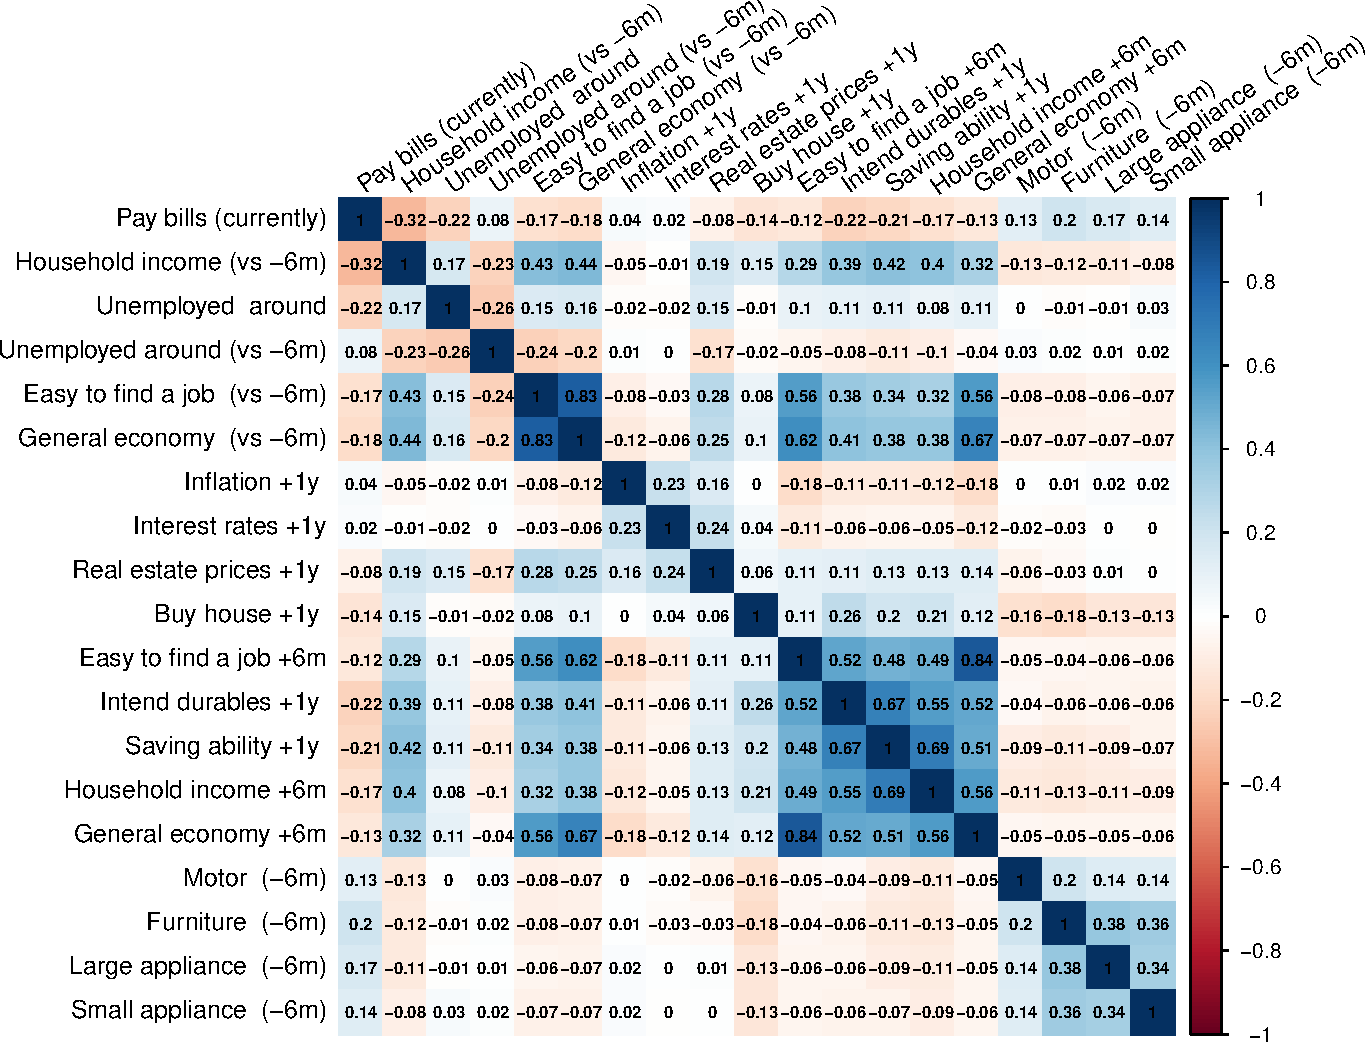
\includegraphics[width = 425pt]{icc_item_correlation.pdf}
\end{figure}


\begin{table}[]
  \caption{Items in detail (I)} 
  \label{item_table_1} 

 \begin{tabular}{  | p{5cm} | p{5cm} | p{5cm} |}
\hline
\multicolumn{1}{|l|}{Item short name}       & \multicolumn{1}{p{8cm}|}{Complete question}                                                                                                                   & \multicolumn{1}{p{3.5cm}|}{Response options} \\ \hline \hline
\multicolumn{1}{|p{4cm}|}{Motor (-6m)}           & \multicolumn{1}{p{8cm}|}{\emph{In the last six months, have you, or someone in your household, acquired any of the following goods: car or motorbike?}}              & \multicolumn{1}{p{3cm}|}{Yes/No}           \\ \hline
\multicolumn{1}{|p{4cm}|}{Furniture (-6m)}       & \multicolumn{1}{p{8cm}|}{\emph{In the last six months, have you, or someone in your household, acquired any of the following goods: household furniture?}}               & \multicolumn{1}{p{3cm}|}{Yes/No}           \\ \hline
\multicolumn{1}{|p{4cm}|}{Large appliance (-6m)} & \multicolumn{1}{p{8cm}|}{\emph{In the last six months, have you, or someone in your household, acquired any of the following goods: large appliance or a computer?}} & \multicolumn{1}{p{3cm}|}{Yes/No}           \\ \hline
\multicolumn{1}{|p{4cm}|}{Small appliance (-6m)}       & \multicolumn{1}{p{8cm}|}{\emph{In the last six months, have you, or someone in your household, acquired any of the following goods: small household appliance?}}               & \multicolumn{1}{p{3cm}|}{Yes/No}           \\ \hline
\multicolumn{1}{|p{4cm}|}{Unemployed  around}       & \multicolumn{1}{p{8cm}|}{\emph{How many people in your environment are currently unemployed and looking for a job?}}               & \multicolumn{1}{p{3cm}|}{Integer}           \\ \hline
\multicolumn{1}{|p{4cm}|}{Unemployed around (vs -6m)}       & \multicolumn{1}{p{8cm}|}{\emph{Compared to six months ago, are there more or less people in your environment are currently unemployed and looking for a job?}}  & \multicolumn{1}{p{3cm}|}{More/Same/Less}           \\ \hline
\multicolumn{1}{|p{4cm}|}{Easy to find a job  (vs -6m)}       & \multicolumn{1}{p{8cm}|}{\emph{Do you think the situation to find a job in Spain is now better or worse than six months ago?}}  & \multicolumn{1}{p{3cm}|}{Better/Same/Worse}           \\ \hline
\multicolumn{1}{|p{4cm}|}{Pay bills (currently)}       & \multicolumn{1}{p{8cm}|}{\emph{Which of the following assertions describes best the economic situation of your household?}}  & \multicolumn{1}{p{3.5cm}|}{From 1- \emph{``Struggle to pay bills and have to take debt''} to 5- \emph{``Get easily to the end of the month and manage to save''} }           \\ \hline
\multicolumn{1}{|p{4cm}|}{Household income (vs -6m)}       & \multicolumn{1}{p{8cm}|}{\emph{Do you consider that the current economic situation of your household is now better or worse than six months ago?}}  & \multicolumn{1}{p{3cm}|}{Better/Same/Worse}           \\ \hline
\multicolumn{1}{|p{4cm}|}{General economy  (vs -6m)}       & \multicolumn{1}{p{8cm}|}{\emph{Do you consider that the current Spanish economic situation to be now better or worse than six months ago?}}  & \multicolumn{1}{p{3cm}|}{Better/Same/Worse}           \\ \hline




\end{tabular}
\end{table}


\begin{table}[]
  \caption{Items in detail (II)} 
  \label{item_table_2} 

 \begin{tabular}{  | p{5cm} | p{5cm} | p{5cm} |}
\hline
\multicolumn{1}{|l|}{Item short name}       & \multicolumn{1}{p{8cm}|}{Complete question}                                                                                                                   & \multicolumn{1}{p{3.5cm}|}{Response options} \\ \hline \hline
\multicolumn{1}{|p{4cm}|}{Easy to find a job +6m}       & \multicolumn{1}{p{8cm}|}{\emph{Do you consider that the situation to find a job in six months will be better or worse than in the present?}}  & \multicolumn{1}{p{3cm}|}{Better/Same/Worse}           \\ \hline
\multicolumn{1}{|p{4cm}|}{Intend durables +1y}       & \multicolumn{1}{p{8cm}|}{\emph{Do you consider that the probability that you acquire consumer durables (cars, furniture, appliances, computer, but excluding real estate) in the coming year will be better or worse compared to the present year?}}  & \multicolumn{1}{p{3cm}|}{Higher/Same/Lower}           \\ \hline
\multicolumn{1}{|p{4cm}|}{Saving ability +1y}       & \multicolumn{1}{p{8cm}|}{\emph{Do you consider that your capacity to save during the coming year will be better or worse, compared to the present year?}}  & \multicolumn{1}{p{3cm}|}{Better/Same/Worse}           \\ \hline
\multicolumn{1}{|p{4cm}|}{Household income +6m}       & \multicolumn{1}{p{8cm}|}{\emph{Do you consider that the economic situation of your household during the next six months, will be better or worse, compared to the present year?}}  & \multicolumn{1}{p{3cm}|}{Better/Same/Worse}           \\ \hline
\multicolumn{1}{|p{4cm}|}{General economy +6m}       & \multicolumn{1}{p{8cm}|}{\emph{Do you consider that the economic situation of Spain during the next six months, will be better or worse, compared to the present year?}}  & \multicolumn{1}{p{3cm}|}{Better/Same/Worse}           \\ \hline

\multicolumn{1}{|p{4cm}|}{Buy house +1y}       & \multicolumn{1}{p{8cm}|}{\emph{Do you personally have plans to buy a house in the coming year?}}  & \multicolumn{1}{p{3cm}|}{Yes/No}           \\ \hline
\multicolumn{1}{|p{4cm}|}{Inflation +1y}       & \multicolumn{1}{p{8cm}|}{\emph{The increase of prices (or inflation) during last year has been of XXX. Do you think that in the coming year prices will grow faster, or more slowly than in the past year?}}  & \multicolumn{1}{p{3cm}|}{Faster/Same/More slowly}           \\ \hline
\multicolumn{1}{|p{4cm}|}{Interest rates +1y}       & \multicolumn{1}{p{8cm}|}{\emph{Do you think that in the coming year,  the interest rate at which financial institutions give loans will either increase or decrease?}}  & \multicolumn{1}{p{3cm}|}{Increase/Stay the same/Decrease}           \\ \hline
\multicolumn{1}{|p{4cm}|}{Real estate prices +1y}       & \multicolumn{1}{p{8cm}|}{\emph{Do you think that in the coming year,  real estate prices will either increase or decrease?}}  & \multicolumn{1}{p{3cm}|}{Increase/Stay the same/Decrease}           \\ \hline
\end{tabular}
\end{table}




\end{document}